\chapter{Dall'analisi all'operatività: il paper trading}
\label{ch:paper-trading}

\section{Motivazione}
\label{sec:live-motivazione}

Un backtest, per quanto rigoroso, resta una simulazione condotta su dati
storici. Fra una strategia che funziona sui dati passati e un sistema capace
di operare autonomamente in tempo reale esiste una distanza fatta di
problemi che il backtest non pone: l'autenticazione all'exchange, il recupero
e la validazione dei dati di mercato in tempo reale, la gestione dello stato
tra un ciclo e il successivo, la traduzione di un segnale in un ordine
concreto. Per colmare questa distanza, e per verificare la replicabilità
operativa dell'intera pipeline, la strategia è stata implementata in un
sistema di paper trading che opera sulla testnet di Deribit. Questo capitolo
ne descrive l'architettura e la coerenza con il backtest.

\section{Architettura del sistema}
\label{sec:live-architettura}

Il sistema di trading in tempo reale si compone di quattro moduli, orchestrati
da un ciclo eseguito periodicamente. Il primo modulo è il client
dell'API REST di Deribit, che gestisce l'autenticazione OAuth2, il refresh
del token e le chiamate agli endpoint di mercato e di trading, con la
possibilità di operare indifferentemente su testnet o in produzione. Il
secondo modulo è lo \emph{scorer}, che replica in tempo reale la logica di
selezione Top Vega sulla catena di opzioni corrente, applicando gli stessi
filtri del backtest (opzione a vega massimo, out-of-the-money, con delta
entro la soglia e scadenza nell'intervallo ammesso). Il terzo modulo è il
\emph{position manager}, che tiene traccia delle posizioni aperte, verifica
le condizioni di uscita e persiste lo stato su file, così da sopravvivere ai
riavvii del processo. Il quarto modulo è l'\emph{order executor}, che
traduce le decisioni in ordini e che, qualora l'autenticazione fallisca,
ripiega automaticamente in modalità \emph{dry-run}, simulando l'esecuzione
senza inviare ordini reali.

Il ciclo di trading, eseguito a intervalli regolari, procede nell'ordine:
recupero e scoring della catena di opzioni, verifica delle condizioni di
uscita sulla posizione eventualmente aperta, ribilanciamento della copertura
delta, e infine, se non vi sono posizioni aperte, apertura di una nuova
posizione sull'opzione selezionata. Al termine di ogni ciclo lo stato viene
salvato.

La Figura~\ref{fig:ciclo-live} schematizza il ciclo.

\begin{figure}[H]
\centering
\begin{tikzpicture}[
  node distance=5mm and 7mm,
  box/.style={rectangle, rounded corners=2pt, draw=black!70, fill=black!4,
              minimum height=9mm, minimum width=24mm, align=center, font=\small},
  arr/.style={-{Stealth[length=2.5mm]}, thick, black!70}
]
\node[box] (fetch)   {Fetch\\option chain};
\node[box, right=of fetch] (score)   {Scoring\\Top Vega};
\node[box, right=of score] (exit)    {Verifica\\condizioni exit};
\node[box, right=of exit]  (hedge)   {Ribilanciamento\\hedge delta};
\node[box, below=9mm of hedge] (entry)   {Apertura nuova\\posizione};
\node[box, left=of entry]  (persist) {Persistenza\\stato};
\draw[arr] (fetch) -- (score);
\draw[arr] (score) -- (exit);
\draw[arr] (exit) -- (hedge);
\draw[arr] (hedge) -- (entry) node[midway, right, font=\scriptsize] {se flat};
\draw[arr] (entry) -- (persist);
\draw[arr] (persist.west) to[out=180, in=270]
  node[midway, below left, font=\scriptsize] {ciclo ogni 4 ore} (fetch.south);
\end{tikzpicture}
\caption{Il ciclo di trading del sistema live: recupero e scoring della
catena di opzioni, verifica delle uscite, ribilanciamento della copertura,
eventuale apertura di una nuova posizione e persistenza dello stato.}
\label{fig:ciclo-live}
\end{figure}

\section{Coerenza tra backtest e sistema live}
\label{sec:live-coerenza}

Il sistema live condivide con il backtest le regole, i parametri e la logica
di dimensionamento (configurazione moderata, rischio 2\% con buffer
1,5$\times$), attingendo alla stessa configurazione centralizzata. Restano
alcune differenze inevitabili tra i due contesti. Il backtest esegue con
tempistica T+1 giornaliera, mentre il sistema live opera a intervalli
infragiornalieri; il profitto della copertura, calcolato nel backtest sui
prezzi di chiusura dei futures trimestrali, nel sistema live va ricostruito
dai prezzi in tempo reale, accumulandolo tra un ciclo e il successivo.

Proprio quest'ultimo punto ha offerto una lezione operativa. Durante il
paper trading è emerso che il profitto della gamba di copertura non veniva
accumulato correttamente da un ciclo all'altro: il sistema tracciava la
posizione di copertura ma non consolidava la variazione di valore tra i
prezzi successivi del futures. Il problema è stato individuato e corretto,
introducendo un tracciamento esplicito del prezzo di copertura e
dell'accumulo del relativo profitto tra i cicli. È un esempio del tipo di
difetto che solo l'esecuzione in condizioni reali fa emergere, invisibile in
un backtest in cui l'intera storia dei prezzi è disponibile simultaneamente.

\section{Monitoraggio}
\label{sec:live-monitoraggio}

Il sistema è corredato da una dashboard di monitoraggio, mostrata nella
Figura~\ref{fig:live-dashboard}, che visualizza in tempo reale la posizione
corrente, le greche, lo stato della copertura, il profitto non realizzato e
lo storico dei trade, oltre al confronto tra la curva di equity live e
quella attesa dal backtest.

\begin{figure}[H]
\centering
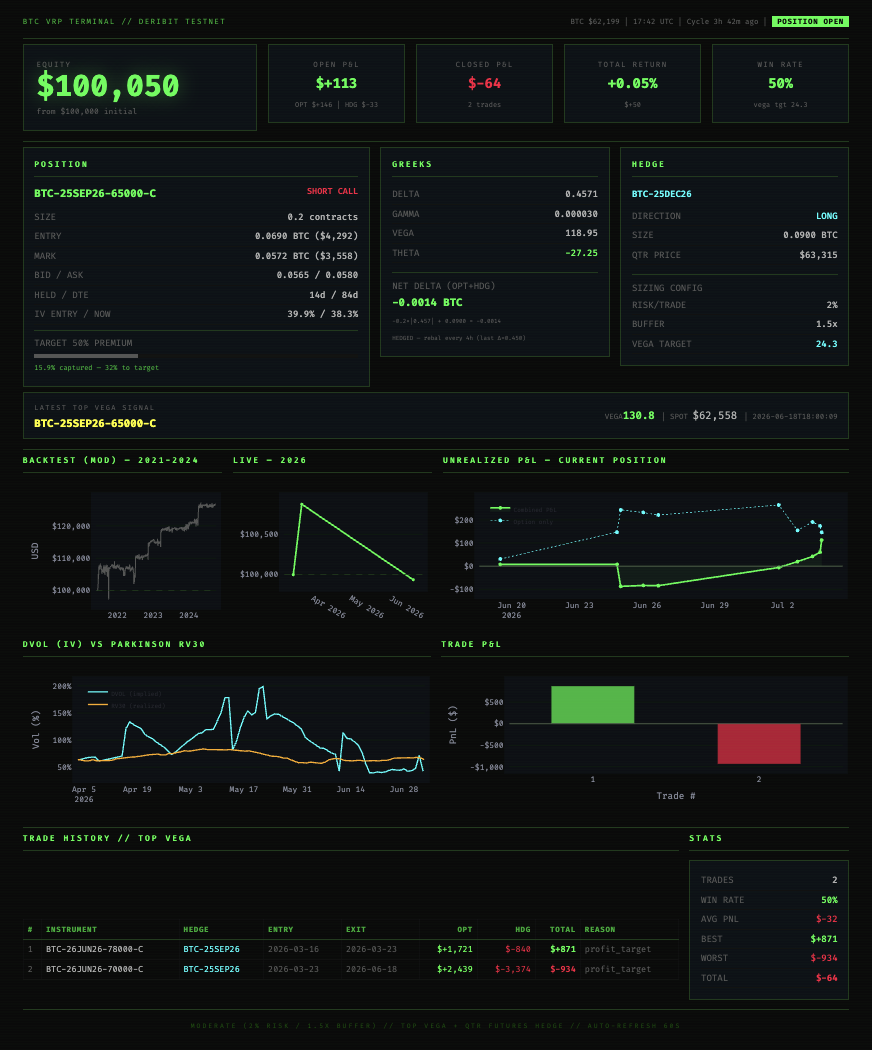
\includegraphics[width=0.8\textwidth]{figures/screen-dashboard-030702026.png}
\caption{Dashboard di monitoraggio del paper trading (testnet Deribit,
3 luglio 2026): posizione corrente e greche, stato della copertura con
futures trimestrali, segnale Top Vega più recente, confronto tra curva
di equity del backtest e curva live, profitto non realizzato della
posizione aperta e storico dei trade chiusi.}
\label{fig:live-dashboard}
\end{figure}

Alla data di questa stesura (luglio 2026) il sistema ha completato due
trade e detiene una terza posizione aperta: un campione ancora
insufficiente per qualunque valutazione statistica. I risultati
quantitativi del paper trading, con il confronto sistematico tra curva
live e curva attesa dal backtest, saranno consolidati nella versione
finale del lavoro, al termine del periodo di osservazione.
